% Hewitt  - Application Design  - Standards and policies
% Hewitt  - Application Design  - Guidelines and conventions
% Smith  - Requirements  - Specific System Description  - Problem Description  - Goal Statements
% ICD Interface Control Document
% Smith  - Requirements  - General System Description  - System Constraints

%\newcommand{\red}{\color{red}}
%\newcommand{\blue}{\color{blue}}
%\newcommand{\green}{\color{green}}
\newcommand{\red}{\itshape}
\newcommand{\blue}{\itshape}
\newcommand{\green}{\itshape}

%\clearpage

%This section provides a response to Tokamak Science's exhaust code
%requirements document.
\newsectionnobreak{Response to Tokamak Science Division}{sec:response_physics}
\subsection{Introduction}
\label{sec:introduction}

This section is Project \nep's response to Tokamak Science and MAST Upgrade Division's
Requirements Specification document.
This specification was received by Wayne Arter  on 5/11/20 via Rob Akers
and its authorship was confirmed to be Fulvio Militello and James Harrison at the \nep \  Project Board.
It is intended that this document helps to frame expectations of the
capabilities of \nep\ code,
as well as highlighting challenges and areas of potential collaboration.
Since  the main focus herein is on aspects of the physical model, the
next \Sec{TS_sw_response} goes into more detail regarding the software engineering
needed to deliver the code successfully.

The physics requirements are summarised as:
\begin{quote}
``The new UKAEA Exhaust code needs to be able to capture parallel and
perpendicular transport of charged and neutral particles in 3D, full geometry
and in a time dependent way. Turbulence should be self-consistently modelled,
as well as energy transfer physics between charged particles, neutrals and
photons (radiation). While perturbations need to be 3D, a minimal requirement
for the code is that it can simulate realistic axisymmetric equilibrium
configurations with complex topologies and wall designs.
The aim of the code should be to:
\begin{enumerate}
	\item Efficiently and reliably model exhaust in next generation
		experiments, like eg.\  MAST-U, JT60-SA, and especially ITER
		(the latter is a stringent requirement for the code).
	\item Allow predictive exhaust capability for future reactor relevant
		machines like STEP or DEMO.''
\end{enumerate}
\end{quote}
More detailed specifications are given in the following sections
either as block quotations or as bold paragraph headers.

\subsubsection{\nep\ Science Plan}

The Science Plan for \nep\ \cite{sciplan} is available
online.
The stated goal of the project is to:
{\green 
\begin{quote}
	``develop new algorithms, software and related e-Infrastructure that will result in the efficient use of current Petascale and future Exascale supercomputing hardware in order to
\begin{enumerate}
	\item draw insights from ITER ``Big Data''
	\item to guide and optimise the design of the UK demonstration nuclear
		fusion power plant STEP and related fusion technology
\end{enumerate}
in the approach to the Exascale. The aims of the work are to deliver expertise in,
and tools for, ``in-silico'' reactor interpretation and design.''
\end{quote}}

The Science Plan also describes the software development and theory development
that is being and will be undertaken under \nep.

\paragraph{Software development.}
The aim of \nep\ software development is to provide a flexible framework for
implementing different physical models in an Exascale-targeted manner.
In particular, the project does \emph{not} envisage a ``\nep\ system of equations'' so
much as \nep\ providing the ability to solve a class of relevant equations,
with models described relatively simply using a Domain-Specific Language (DSL).
This flexibility enables the hierarchy of models of varying fidelity and
computational costs.
It also allows engagement from different classes of user with different levels
of physics and software expertise.

\paragraph{Theory development.}
The above framework approach notwithstanding,
\nep\ is also supporting theory development in two of its four work packages:
FM-WP2 Plasma Multiphysics Model and FM-WP3 Neutral Gas and Impurity Model.
These will develop two close coupled models, with FM-WP2 seeking to include
kinetic effects in existing and new edge plasma models, and FM-WP3 developing
particle-based models for describing the region outside and just inside the
plasma (neutral atoms/molecules and partially ionised impurities).

Another work package, FM-WP1 Numerical Representation, is addressing related
numerical issues, such as
the accurate modelling of highly anisotropic dynamics,
the accurate representation of first wall geometry,
and the numerical preservation of conservation laws from the underlying models.

As such the \nep\ plan is aligned with all the points in the summary
requirements quoted above, though there are minor issues regarding
the details as discussed in the following sections.
It should be noted that the Science Plan outlines a five-year programme that
explicitly requires user involvement for fuller development of surrogate
models (such as turbulent friction) and to specify the detailed physics of
ionisation and excitation reactions.
It follows that development of many of the physics capabilities listed below will benefit
greatly from a strong collaboration between
Tokamak Science and Advanced Computing.

\subsection{Overall Capabilities}
\label{sec:capabilities}

\subsubsection{Hierarchical approach with multiple models}

``Hierarchical approach with multiple models, going from low fidelity
(eg.\  laminar fluid and fluid-kinetic runs in 2D) to medium fidelity (eg.\ 
fluid runs with neutrals and turbulence  multispecies, but with reduced number
of species) and high fidelity (eg.\  full kinetic or hybrid kinetic/fluid runs
with turbulence and multispecies approach).''

The plan is for \nep\ to provide a framework for solving relevant physics
models, and a user-friendly Domain-Specific Language (DSL) for doing this.
This allows UKAEA to develop its own physics models in a manner significantly
independent of \nep\ development and code distribution, see \Fig{proxyflow2}.
This is the same approach as currently used by UKAEA for BOUT++,
where UKAEA has ownership of physics models in the STORM software, while other organisations have
ownership of the BOUT++ framework.

Project \nep \ intends to provide a suite of examples of physics models as part of the code
distribution.
As addressed in \S\ref{sec:physics_model}, there is also development of a
physics model under \nep\ that could be adaptive, displaying a range
of fidelities within different regions of the domain during a single
simulation.

\begin{figure}
\centerline{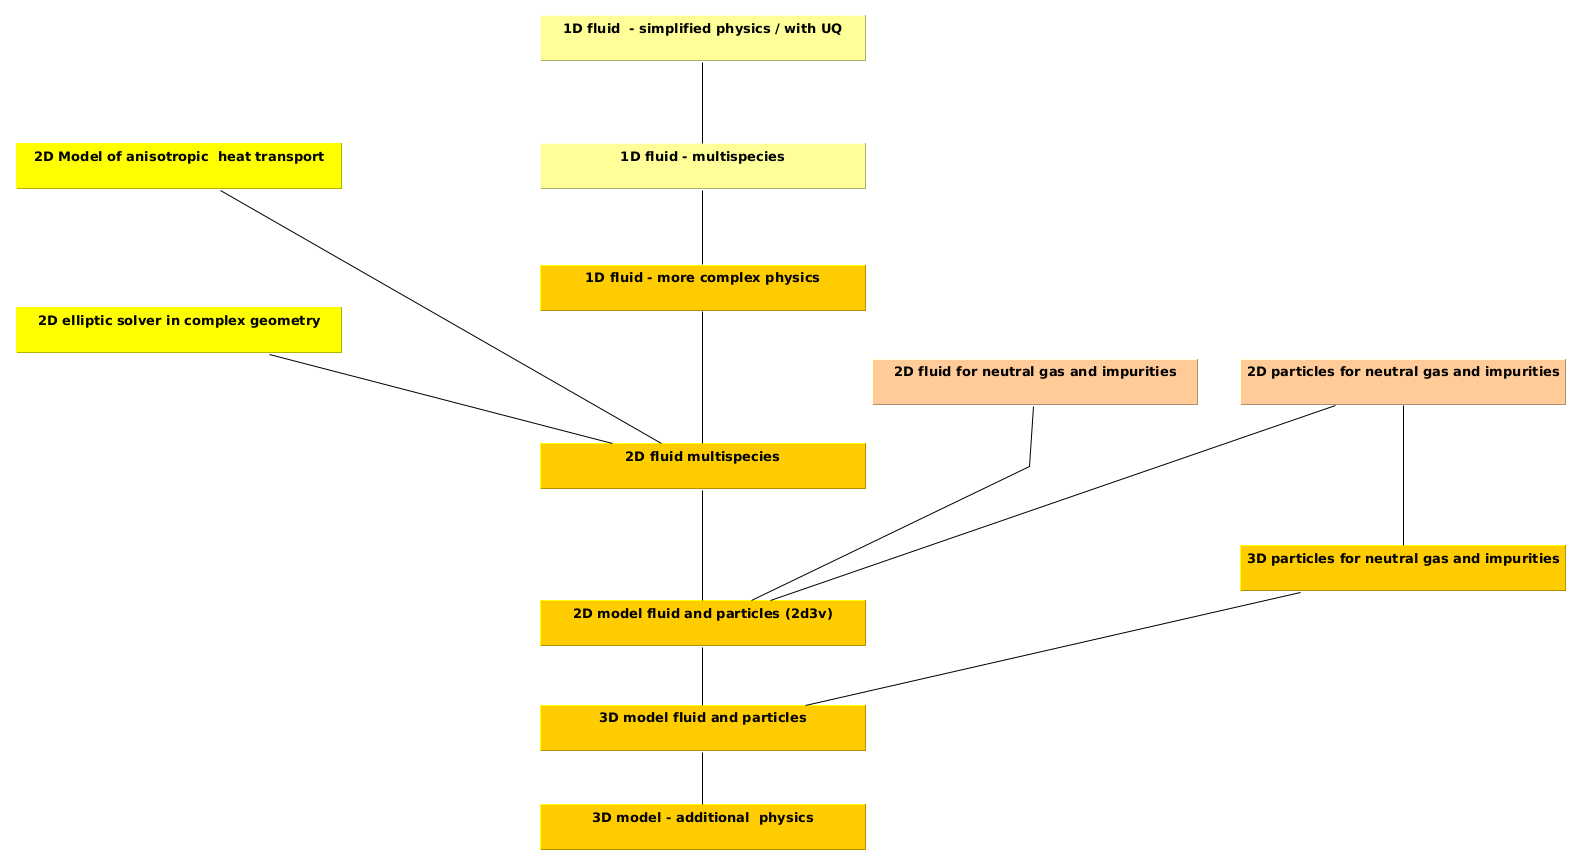
\includegraphics[width=0.95\textwidth]{./pics/proxyflow2.png}}
\caption{
Development of \nep \ software via a sequence of \papp s.
\label{fig:proxyflow2}}
\end{figure}

\subsubsection{Numerical efficiency}

``Numerical efficiency obtained for example through scalability to
large number of cores (given the expected computational resources, the
code should be designed to take: $\sim$1 week for low fidelity
parametric scans; $\lesssim$1 month for medium-high fidelity runs for
advanced design; $\lesssim$3 months for high fidelity physics studies).''

Order of magnitude estimates for the cost of code execution (see~\Sec{cg}),
indicate that these timings are possible but challenging.

The plan is to target Exascale simulations that can support high-fidelity physics
simulations.
Project \nep \ aims to do this in a performance portable fashion using abstraction
layers to separate the physics from the computation details.
However, the challenges of Exascale mean that a degree of
specialisation of the code towards available Exascale machines is expected.
At some point this will probably entail trade-offs that are detrimental to
performance on smaller machines.
Despite this, we still anticipate that the software
should be reasonably performant for small-scale runs.

\subsubsection{Stability of the code}

``Focus on stability of the code, using (preferably) unconditionally
stable numerical schemes and capability to diagnose and re-start failed runs.
Ensure a small failed simulation rate for common configurations.''

The focus will be on accuracy rather than stability.
An accurate solution will be a stable one, whereas the converse is not true.
The use of bifurcation tracking techniques is expected to help with numerical
stability. 
Moreover, the use of ensemble techniques (as part of uncertainty quantification)
should provide information on stability as a function of parameters, as well as
making it likely that at least a subset of calculations produces usable
results.

In addition, there are some planned technical solutions for diagnosing problems
with runs.
The simplest functionality is to allow users to change parameters when
restarting a job using checkpoint files.
The code can also be made to automatically check input files (to catch user
misspellings), and to output a file containing the parameters that were
actually used in a simulation (in case some were accidentally overwritten).
Simulations may also be given a Universally Unique Identifier (UUID) to allow
provenance tracking of simulations.


\subsubsection{Exhaust physics modelling capability}

``Provide capability to model exhaust physics all the way from sheath
limited to strongly detached regimes.''

This capability follows from (1) the implemented physics models/boundary
conditions, and (2) the lengthscales the code can resolve in simulations of
feasible run times.
Project \nep \ anticipates that this will be feasible. 
See \S\ref{sec:physics_model} for further details for the physical
models.


\subsubsection{Modern software design}

``Modern software design with modular approach (independent and efficient libraries).''

Project \nep \ is certainly adopting a modular approach to software design.
This is crucial for enabling many of the desired features, as noted below.
The use of reliable third-party libraries is also vital for enabling a small
team of developers to leverage the work of others, and to allow code
flexibility and ease of prototyping.

\subsubsection{Ability to integrate with other codes (eg.\ with IMAS).}
This feature is anticipated, and will be facilitated by writing the code in
object-oriented C++.

Integration with IMAS (and other data formats/standards) can be achieved by
writing a module to translate between \nep's internal data structures and IMAS
format.
\nep\ developers are involved in TSVV software which will also integrate with
IMAS, so will have experience in this area.

\subsubsection{Modern visualisation tools}
Integration with modern visualisation tools is not specifically addressed in
the science plan.
However, this is enabled by using standard data formats such as netCDF/HDF5.
Auxiliary tools (similar to BOUT++'s xBOUT library) could also be developed.

The issue of \emph{in situ} visualisation will also be important at the Exascale,
with the need to interrogate large quantities of data without moving it,
perhaps during a simulation.
Project \nep \ does not have specific plans for enabling this.
However, the need for this will be widespread, and we expect third-party
tools/libraries to become available to support this, particularly in C++.

\subsubsection{Accessibility (output easily catalogued and interrogated  big data)}
Given the constraint of producing Exascale volumes of data,
it is expected that \nep\ will default to using the Met Office practice of only
saving the files necessary for repeating a simulation, rather than full
outputs.
It is intended that key aspects will be captured by surrogates, descriptions of
which will be saved and indexed.
Users however will be able to choose to output more data and to define
custom diagnostics.
A modular approach to software design and the use of standard libraries will
ease the implementation of these.

In time, there will likely be a move towards creating
simulation databases in preference to repeating expensive simulations.
Such projects are nascent, but we have collaborators who are working in this
area.
Again, the modular approach and use of standard data structures will enable
interfacing with such databases as the technology matures.

% WA: It is expected that we shall adopt Met Office practice and only save the
% files needed to repeat simulations, rather than full outputs. It is intended
% that key aspects will be captured by surrogates, descriptions of which will
% be saved and indexed.
% JTP: Outputting more would be a user option though?

\subsubsection{Version control and user support.}
Version control is a fundamental part of modern software development, and will
certainly be used in \nep.
More generally, the project will use best software practices, including
protected branches, peer reviewed pull requests, issue trackers and automated
testing.
The main code contributors are familiar with such practices; we have heavy
involvement from the projects BOUT++ and Nektar++ which have very high quality
software practices.
Project \nep \ also have involvement from UKAEA RSEs.

User support will be provided through issue trackers, a project Slack channel,
and where relevant, through training sessions.
Project \nep \ anticipates supporting several classes of user, from
those with limited software knowledge,
to users with appreciation of different numerical/algorithm choices,
through to numerical/software specialists who might edit the code on a granular
level.
Support for such a wide range of uses is enabled by a highly modular
separation-of-concerns approach.


\clearpage
\subsection{Physics model}
\label{sec:physics_model}

\subsubsection{General requirements}

\begin{quote}
``Equations need to be applicable to arbitrary aspect ratio devices.''
\end{quote}

The equations employed will not generically make the assumption of small
inverse aspect ratio.

\begin{quote}
The collision operators between plasma components, plasma and
impurities and plasma and neutrals have to be sufficiently accurate to properly
describe the radiation generated and the energy transfer between species.
\end{quote}

These operators may be included in the model being
derived in FM-WP2, but at this stage simpler model operators are being used.

\begin{quote}
``Photon opacity effects need to be included in the model.''
\end{quote}

The treatment of effects due to radiation are discussed in Annex~A of ref~\cite{pappeqs2}
(``the equations document"). Initial implementation will account only for
usage~(1) \emph{the calculation of source/loss terms}, with usage~(2) \emph{the production
of synthetic spectra}, depending very much on input from experimentalists,
as anticipated in the science plan~\cite[p\.\,11]{sciplan}.

\begin{quote}
``The equations need to be capable of dealing with multiple species in
non-trace amounts (at least D, T, He and seeding impurities).''
\end{quote}

The models being derived support distribution functions for multiple species.

\begin{quote}
``The equations should not rely on the Boussinesq approximation.''
\end{quote}

The model derived in FM-WP2 does not use the Boussinesq approximation.
Technically, this means \nep\ will need to be able to invert three-dimensional
elliptic operators with non-constant coefficients.
This capability will be available.

\begin{quote}
``The code should evolve both the electron and ion energy (temperature).''
\end{quote}
This is the case with the FM-WP2 model.

\begin{quote}
``It would be acceptable to have only axisymmetric equilibria,
potentially corrected through small perturbations.''
\end{quote}
This is answered by the discussion in \Sec{geometry}.


\subsubsection{High fidelity simulations}
\begin{quote}
``In high fidelity simulations, the kinetic/fluid transition for both plasma and
neutrals has to be properly captured, potentially using a multi-region approach
exploiting different models in different parts of the machine could be
considered (for both neutrals and plasma);
Boundary conditions need to consider improved sheath physics (collisional \&
shallow angles);
Ideally, the model should be able to treat de-magnetized ions in the divertor
region;
Electromagnetic effects should be included, but a perturbation approach would
be acceptable.''
\end{quote}

The Science Plan states that {\green ``FM-WP2 and FM-WP3 will concentrate upon
development of the two close coupled models of the \nep \  programme,
specifically FM-WP2 around the inclusion of kinetic effects into existing and
new edge plasma models, and FM-WP3 of particle based models for describing the
region outside and just inside the plasma (neutral atoms/molecules and
partially ionized impurities).''} See \Fig{colpri}.

\begin{figure}
\centerline{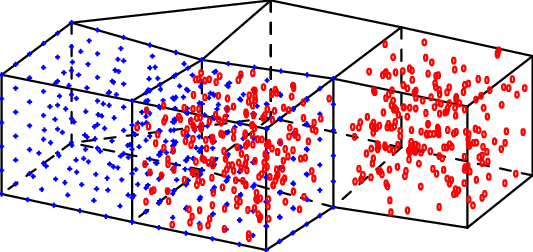
\includegraphics[width=0.7\textwidth]{./png/colpri.png}}
\caption{
\nep \ software will use finite elements and particles to represent different atomic species
as needed.
\label{fig:colpri}}
\end{figure}

In FM-WP2, a novel ``moment-based'' approach is being developed (for both
plasma species and neutrals).
This approach is a variant on gyrokinetics (though at present, the derivation
exists only for drift kinetics).
Instead of the stationary background Maxwellian of the usual gyrokinetics, this
approach uses a dynamically-varying background Maxwellian, where the
particle density, bulk velocity and temperatures are allowed to vary with time.
The result is a hybrid approach, where the software evolves both a fluid system
and a modified kinetic system.
One of the benefits of this approach is that it gives a natural means to
capture the fluid/kinetic transition, by switching between the fluid+kinetic
and fluid-only descriptions.
Moreover this approach allows the software to detect which of the fluid and kinetic
descriptions is valid in any region based on the properties of the modified
distribution function, and therefore to automatically evolve the relevant
model.

The favourable properties of this approach are valuable,
but as with any novel approach there is an inherent risk of the scheme not
working.  Thus as described in ref~\cite[\S\,1.1]{pappeqs2}, in the event that
this approach is not feasible, the kinetic calculations
will use a Particle-in-Cell (PIC) approach.
While full orbit PIC is potentially extremely expensive relative to gyrokinetics,
it has been very well-studied both in terms of theory and numerical implementation.
Moreover the issue of how to treat the transition from fluid to a particles in
a coupled model is well-understood, at least in classical fluid dynamics.

Relevant sheath physics boundary conditions are being derived as part of this
work, including shallow angles and collisions.
Ions which exit the domain re-enter as neutrals with the Knudsen cosine
distribution.

While the current derivation is electrostatic, there is nothing which precludes
the derivation of an electromagnetic model.


\subsubsection{Neutrals and impurities}

\paragraph{Different levels of multispecies capabilities should be considered.}
The framework nature of the code means this will be the case.

\paragraph{In medium to high fidelity models, neutrals and heavy species should
be treated fully kinetically (the former have potentially low collisionality
and they are not bound by the magnetic field, the latter have a large Larmor
radius).}

Development of a neutral gas and impurity model is ongoing under FM-WP3. 
Page 7 of the Science Plan states: {\green ``Kinetic levels of complexity are \ldots
necessary \ldots for modelling the burning plasma regime, due to the inherent
uncertainty in the fluid codes. 
The plasma in a fusion reactor may well behave significantly differently to
plasma in existing devices because it will in general contain two main ionic
species (Deuterium and Tritium), neutral fuel particles and ionised Helium ash
(or alpha particles), as well as impurity ions originating from the wall.''}
That is, kinetic models will be derived and implemented, though it is hoped
that this will facilitate the development of fluid models.

\paragraph{In high fidelity models, dynamical neutral evolution on the
turbulence time scale would be preferable, if possible.}
High-fidelity simulations will use a kinetic model for neutrals where appropriate. 

\paragraph{Ability to model pumps (either directly or via pumping surfaces)
should be included. Pellets: the code should enable simulation of, or coupling
to models that can model, pellet fuelling.}
Models for these aspects are not included in the Science Plan.
As we will use an unstructured mesh, it will be possible to describe arbitrary
pumping surfaces.

The role of sources and sinks is recognised to be crucial in \nep\ physics so
that modelling of pellets as a source will be possible.
The tool CWIPI (Coupling With Interpolation Parallel Interface) may be used for
coupling to more complicated pellet models.

\clearpage
\subsection{Physics capabilities}
\label{sec:physics_capabilities}

``The code needs to be able to give reliable predictions of:
\begin{itemize}
\item[$\bullet$] Divertor loads:
\begin{itemize}
\item[$\bullet$] Reliable calculation of upstream particle and heat flux
	profiles: proper drift physics and upstream turbulence;
\item[$\bullet$] Divertor turbulence: turbulence spreading in the divertor
	region, effect of magnetic shear next to the X-point(s) to understand
	upstream/downstream connection;
\item[$\bullet$] Multifluid capacity to model radiation and detachment physics;
\item[$\bullet$] Reliable calculation of the electric field (collisionless
	physics near the separatrix, proper reflection of neutrals at the
	target);
\item[$\bullet$] Able to capture in/out and top/down asymmetries (geometry,
	drifts, radiation and detachment)
\end{itemize}
\item[$\bullet$] Wall loads:
\begin{itemize}
\item[$\bullet$] Should be able to predict filamentary transport and role of
	hot ion confinement (wall erosion)
\item[$\bullet$] Should calculate radiation and neutral loads (may require
	dedicated modules, same for divertor loads);
\end{itemize}
\item[$\bullet$] Impurity transport, pumping and fueling:
\begin{itemize}
\item[$\bullet$] Ability to track low (He Be), medium (C, N, Ne) and high Z
	impurities (W, Ar, Xe) with multiple charge states;
\item[$\bullet$] Reliable kinetic modelling of neutrals to assess fueling and
	pumping capacity;
\item[$\bullet$] Ability to handle non-trace species (D, T, He, seeded
	species), which requires new closures for the equations (if fluid,
	beyond Braginskii $\implies$ Zhdanov or better);
\item[$\bullet$] Accurate model of friction forces (turbulence + neoclassical
	on open field lines);
\item[$\bullet$] In high fidelity models, the code should be able to simulate
	localized gas puffs, via injection of neutral particles.
\item[$\bullet$] Dust  the code should enable coupling to codes to simulate
	dust generation, transport and ablation, via exchange of fluxes and
	sources.''
\end{itemize}
\end{itemize}



\paragraph{Physics models.}
Many points in this section relate to the physics model.
As we have alluded to above, the actual physics model used is the
responsibility of the user;
so, for example, it will necessary for users to derive an accurate model for
turbulent friction.
Moreover, as \nep\ will initially be an edge code, only electromagnetic
radiation from the edge plasma will be calculated, and an additional model will
be required for radiation for the core plasma. 
%{\blue Is that what is meant about radiation?}
Nonetheless, we plan to facilitate models which have the listed properties.
In particular, our meshing approach will allow accurate representation of the
walls and divertor.
Thus powerful and flexible source/sink models may be used, for both volumes and
surfaces.

\nep\ code will also be capable of representing scales on which filamentary
transport has been calculated to occur.
The code will only produce fluxes however, and it will be up to the user to
calculate wall erosion.



\paragraph{Validation, Verification and Uncertainty Quantification (VVUQ).}
Naturally, when the solution of a problem is unknown, it is difficult to assess
whether the provided answer is reliable as requested in the first line of the current section.
Therefore we are integrating \nep\ with a suite of tools for VVUQ to enable
validation of code outputs against experimental results, and provide a error
bars for code outputs due to the uncertainty in the code inputs.
As allowed by error estimates, models of different complexity will be used
to predict key properties of the SOL, see \Fig{dimensions2}.
\begin{figure}
\centerline{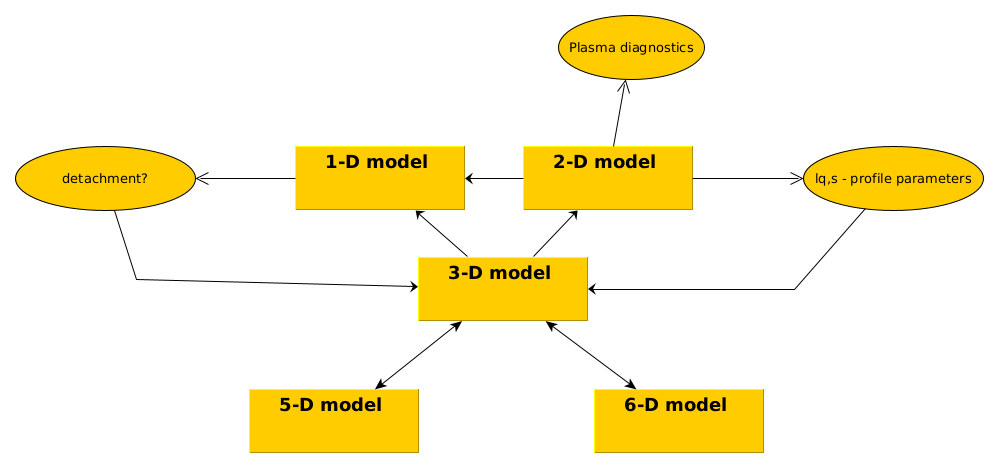
\includegraphics[width=0.7\textwidth]{./pics/dimensions2.png}}
\caption{
Project software will integrate a range of models of different complexity, here
indicated by their dimensionality.
\label{fig:dimensions2}}
\end{figure}

\clearpage
\subsection{Geometry}\label{sec:geometry}

\begin{quote}
``Ability to handle complex topologies and novel geometries:
\begin{itemize}
\item Capacity to treat different topologies with multiple X-points ($>$2),
	possibly in a dynamic way, or at least implemented in a way that does
	not preclude time-varying equilibria being modelled in future; 
\item Ability to handle singularities in the grid (null points) or to develop
	accurate scheme(s) that do not have singularities;
\item Ability to interface with 3D CAD designs of the machine; 
\item Capability to handle conformal grids that go all the way to the wall for
	both neutrals and plasma; 
\item Capability to treat subdivertor structures (only neutrals).''
\end{itemize}
\end{quote}

\nep\ will use a spectral/hp finite element approach.
This allows considerable flexibility in meshing, with elemental tetrahedra,
hexahedra or prisms being used to describe complex geometries.
In addition to refinement of the elemental grid sizes ($h$-adaptivity),
the order of the piecewise polynomial basis functions used on each element may
also be changed ($p$-adaptivity).
The production of finite element griddings conforming to CAD descriptions is standard
for virtually all meshing packages. Project \nep \ will specially aim to use
the small number of packages that may produce finite elements with curved edges and faces 
to exploit fully the higher order basis.
This gives a framework which can achieve spectral convergence on complicated, conforming grids,
while still being able to handle discontinuities in the solution.

%Unlike approaches based on deformations of Cartesian grids
%{\blue (JTP: is this what is meant by conformal mappings here?)},
Should it prove necessary to produce a meshing conforming to
surfaces of an equilibrium magnetic field, then because
the finite element approach does not require a structured grid, it should
be able to treat arbitrary geometries and topologies, 
in particular including multiple X-points.
The approach could be extended by further use of adaptive meshing to allow for time-varying equilibria.

%From the science plan
%\begin{quote}
%	``[NEPTUNE] work will initially focus upon coupling the turbulent plasma periphery
%	to the surrounding neutral gas and partially ionized impurities that
%	exist between the plasma and plasma facing components, in the presence
%	of an arbitrary tokamak magnetic field and full 3-D first wall
%	geometry.''
%
%	``Infrastructure and workflows will be developed so that the resulting
%	close coupled models can be constructed routinely based around a
%	high-fidelity representation of the geometry described by Computer
%	Aided Design (CAD) systems (this likely requiring the development of
%	high order meshing technology, e.g.\ using Nektar++).''
%
%	``P4. Accurate representation of first wall geometry (face normals to
%	within 0.1$^\circ$), and correspondingly of complex magnetic field
%	geometries.''
%
%	Solvers in complex geometries part of ``Plasma multiphysics model
%	(Fusion modelling, work package FM-WP2)''
%
%\end{quote}

\begin{subappendices}
\newsection{Order-of-magnitude estimates for tokamak edge modelling}{sec:cg}
Suppose plasma number density $n \approx 10^{18}$\, m$^{-3}$. Order of magnitude
dimensions are $L\approx0.1$\,m for SOL thickness, reactor minor and major radii
say $a=3$\,m and $R_0=10$\,m, so the volume of SOL $\approx 4 \pi^2 a R_0 L \approx 100$\,m$^3$.
It follows that the total number of electrons $\approx 10^{20}$.

The shortest timescale is inverse $e B/m_e$, the electron cyclotron frequency, where the
ratio of charge to mass for the electron is
$|e|/m_e = 1.76 \times 10^{11}$\,C kg$^{-1}$, and $B\approx 10$\,T, so $\tau_{Be}\approx 10^{-12}$\,s.
Hence the number of particle-steps to evolve $1$\,s of physical time is  $10^{20+12+1}$
(assuming of order $10\pi$~timesteps per orbit),
which assuming $1000$\,flop per update, needs a total of~$10^{36}$\,flop.
Thus to complete a computation in $1$\,s on Exascale machine, only one
$1$~particle-step in $10^{18}$ is allowed.
This implies for example only $100$~superparticles in the volume can be used supposing
each has a weight~$10^{18}$, which
is unlikely to be adequate because electrostatic and other effects will produce a noise level
that swamps any physical effects. However if $3$ or $4$~months (approx.~$10^7$\,s) are allowed, then
a calculation with~$10^9$ particles may be performed if memory-access bandwidth constraints
can be satisfied, when the noise levels may be manageable.

The situation may be shown to be a million times easier for neutrals considered
separately, assuming neutral density~$n_0=n$, particle mass~$m_p$ and temperature~$T_0=10$\,eV, for a
timescale of~$\tau_{0}=L_{mfp}/v_0$ where the mean free path~$L_{mfp}\approx L$ and the neutral
speed typically is~$v_0$. For then $v_0=\sqrt{|e|T_0/m_p}
=\sqrt{|e|/m_e} \cdot \sqrt{m_e/m_p} \sqrt{T_0}$, ie.\ 
$v_{0}\approx 4 \times 10^5 \times (1/40) \times \sqrt{10}\approx 3 \times 10^4$. Thus
$\tau_0\approx 10^{-6}$\,s, ie.\  a million times longer than the electron cyclotron timescale.

Suppose a fluid model is employed instead, ie.\ the electron distribution is
represented by its first~$3$ moments.
If the electron temperature~$T_e \approx 10$\,eV, then the
thermal speed $V_{Te}\approx 40 v_0 \approx 10^6$\,m s$^{-1}$. Supposing the SOL to be sampled at a
uniform~$1$\,mm interval, then the
number of sample-points~$\approx 10^{11}$, and the timestep for an explicit scheme~$\approx (10^{-3} /10^6)\approx 10^{-9}$\,s,
so the number of sample-point updates is $10^{11+9}$. Assuming  $1000$\,flop each update, this
means one second of physical time needs $10^{23}$\,flop or $10^5$\,s$\approx 1$\,d
of Exascale machine time, if memory-access bandwidth constraints can be satisfied. If an implicit scheme
is used to simulate plasma ions as a fluid on a drift type timescale$\approx L/V_{Ti}$, then
possibly the timestep~$\tau_i\approx \tau_0\approx 10^{-6}$\,s, ie.\ a thousand times larger, and
calculations lasting only a few minutes might suffice.

Another way of looking at this is to suppose that numerical problem is $D$-dimensional, $1000$\,flop
are needed for each sample update
and $N_D$~samples per spatial dimension and $N_D^2$ time samples are allowed. Then to update
such a model in $1$\,s requires
$N_D^{D+2} \approx 10^{15}$. Thus  if $D=3$, $N_3 \approx 1\,000$, and $N_5 \approx 100$.
It seems that accuracy controlled, unstructured, implicit fluid models should be possible,
although for the more complex models $1000$\,flop per update may be an underestimate by
orders of magnitude.


\end{subappendices}

\newsection{Software Engineering Response}{sec:TS_sw_response}
The above scientific response~\Sec{response_physics}  indicates that the \nep \ suite
will have the capability to describe the tokamak edge in a 
comprehensive set of levels of detail using a large range of possibly 
heterogeneous computer hardware, will be straightforwardly modifiable to 
include additional physical effects, and will aim to include under all 
circumstances, the level of error in computed results.
Evidently, eveloping the suite represents a major challenge to current software engineering
practices thanks to its scientific difficulty as indicated in \Sec{cg},
and perhaps less obviously, its scientific \emph{complexity} due to the need to treat
large numbers of atomic and molecular species, descending to the level of isotopes
with a range of charge states and electronic excitations.

The last  makes \nep \ a  significantly harder development than the BOUT++ code
discussed in \Sec{response_physics}. The difficulty motivated studies of software
engineering practices outside as well as in the scientific context.
The studies of scientific work are summarised in reports  concerning frameworks,
scientific UQ etc. Ideas from these studies are combined with non-technical works
such as Hewitt~\cite{hewitt} and Sommerville~\cite{sommerville} and
summarised in the report~\cite{y2d34}. 

The outcome is the present report and website, which augment the procedures of
Dudson and BOUT++ collaborators~\cite{y3re314}  to govern the development of \nep.
Management aspects of the development are treated in \Sec{MGT_intro} and
operational aspects in \Sec{OP_MGT}. The remainder of this section focusses
on the generic details of a software implementation, the so-called
non-functional aspects,  with BOUT++ instructions
augmented to allow for the greater complexity of \nep, following the D3.3
reports~\cite{y2d33}, here with~\Sec{TS_varnames} adding a way to handle a multitude of variable
names to accommodate the much increased number of physical variables.
%Conventions
%Latest C++, C++20 if/when possible including modules (like Fortran-95 only import instead of use), and
%concepts - generalised types of single variable.
%Follow Stroustrop~\cite{stroustroptour}, also
%C++ Core Guidelines (Bjarne Stroustrup, Herb Sutter)
%\url{https://github.com/isocpp/CppCoreGuidelines/blob/master/CppCoreGuidelines.md}
%Philosophy section can be condensed to
%\begin{itemize}
%\item Know, and use, available libraries, particularly the Standard Library and the Guideline Support Library.
%\item Also, know, and use, available language features.
%\item Use language to ensure that the purpose of code is unambiguous.
%\item Consider writing a library if none is already available (and presumably making it available to others).
%\end{itemize}

%Use of clang\_tidy, on source code, enforce pot-hole convention.

%Reject unapproved packages

%Two options maintained

%Prepare documents so easy to generate 5-15 slide presentations

%Functionality, expected performance/accuracy, external interface %Smith

Following D3.3~\cite{y2d33}, \Sec{TS_considers} discusses high-level constraints on the structure of software.
where the concept of division into packages and modules (which may represent libraries)  is promoted.
\Sec{TS_scistruct} explores the implications of these constraints for \nep.
At the opposite extreme to \Sec{TS_considers} and \Sec{TS_scistruct},
\Sec{TS_lowlevel} describes the desirable contents for a single module,
and \Sec{TS_procio} discusses the question of what best to output when developing 
software for the Exascale.

\subsection{General Considerations}\label{sec:TS_considers}
It is important that individual units of code are manageable and the overall
structure is comprehensible, so that developers and users can navigate the codebase
and determine where new work is to be located.  This simple consideration implies
that \nep\ software should be divided into units that it will be convenient to refer
to as modules, ie.\ sections of code containing everything necessary to perform one
(and only one) aspect of the desired functionality.

The suggested content of a module
describing a single class in the UML sense (see \Sec{TS_lowlevel}, \Tab{TS_umltrans})
implies a minimum of $13$~methods described by separate subroutines/functions,
with examples extending up to $50$, although the latter is there regarded as an excessively large
number of methods.
Many small software libraries also fall into this size range.
Supposing that each subroutine is of a length to fit within one computer window, ie.\
up to about~$60$~lines, the desirable maximum length of a well-designed module file is
$30\times60 = 1\,800$~lines which is a manageable size of file given 
editing software that remembers on restart, the last line accessed (so that it possible
to return immediately to a particular subroutine).
The magnitude of the D3.3 exercise follows from
the fact that comparable software packages probably of somewhat lesser complexity
than \nep\ written in high level languages such as C++ range in size up to~$1\,000\,000$ lines.
Clearly $400$~separate modules is too unwieldy, and there is a need to organise
further into packages which might contain in turn $10$-$50$ modules. 
As a way of providing further indication to developers,
it is helpful to talk of packages as being arranged into layers, as discussed
in ref~\cite[\S\S\,2.4,3.2]{y2re333}, see \Fig{hierarchygroup}.
Then, as prefigured in ref~\cite[Annex~A]{y2re333}, it should be  possible to encapsulate
the necessary complexity in one, albeit large diagram.
\begin{figure}
\centerline{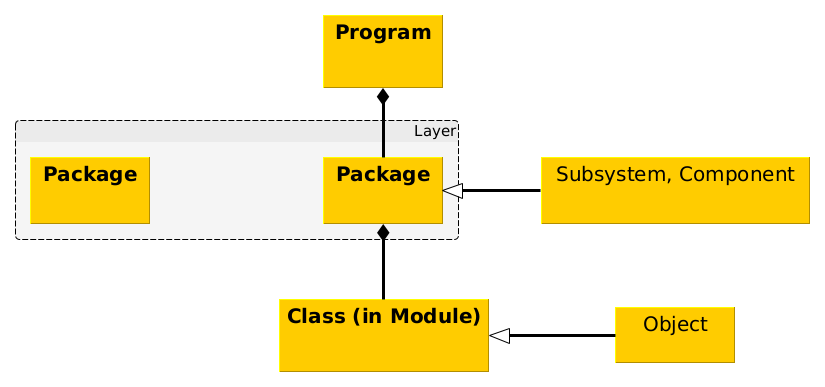
\includegraphics[width=0.7\textwidth]{./png/hierarchygroup.png}}
\caption{
Sketch of relationship between units of large code.
\label{fig:hierarchygroup}}
\end{figure}

\subsection{Considerations for Scientific Software}\label{sec:TS_scistruct}
\subsubsection{Structural Considerations}\label{sec:TS_structure}
In both refs~\cite{y1re331,y2re332}, a figure from Dubey~et~al~\cite{Du16Idea} is reproduced
that illustrates how scientific software may be developed by beginning with an ``infrastructure"
capability into which initially exploratory scientific software is integrated as its worth
is established. Unfortunately for \nep, it is not clear initially what  aspects  of the infrastructure
will be durable and stable, although once the software is more mature, Dubey~et~al's methodology
appears attractive.

The literature referenced in ref~\cite{y2re333}
indicates that scientific software should be produced by aggregation, but is less
helpful as to what is to be aggregated, ie.\  the modular decomposition as to what should
constitute a single module etc.
%Surprisingly little detailed discussion was found in the literature
%after the early book by Booch~\cite{booch}, as to how to create classes in
%the scientific and engineering context, with the exception of Douglass~\cite[\S\,5]{douglass}.
%The ideal would be a way to create classes that enabled rapid development  of code
%that executed efficiently but was easily re-used.
%%where flexibility is also an important consideration,
%Douglass~\cite[\S\,5]{douglass} does not specifically address these last points, but they
%could guide choice of objects in his approach which is reproduced as Appendix~\Sec{TS_objdisc}.

Since the \nep\ development will proceed as a series of \papp s, there is a chance
to refine and redefine an initial modular decomposition with each successive \papp,
recording the results as a UML structure diagram. When generating the corresponding
sequence diagram (ie.\  procedural description), the \papp-based units should be preserved to
facilitate the use of the simpler ones as surrogates for the later more complex \papp s.

To help understand the  aggregation of the software, it should be layered in the obvious manner,
with the higher layers corresponding to greater numbers of aggregated objects. It is also expected
to be useful to classify the modules.
The modules should be arranged into a relatively small number of packages according to, 
eg.\ whether they treat particle generation, matrix coefficient calculation, the main matrix solution, or visualisation.
%\clearpage
\subsubsection{Interactions between Modules}\label{sec:TS_modulint}
Concerning logical interconnections between modules, the 
use of  a directed, acyclic graph~(DAG) structure might be thought mandatory,
particularly to  process the input
data in order to specify coherently the construction of the elements of the solution matrix.
However, as prefigured in ref~\cite{y2re333} for the gyrokinetics code \F{GS2},
the tightly coupled nature of the central edge
physics problem  means that input is more about gathering \emph{all} the data, for only at that point
can fields be computed and only after that may matrix coefficients be computed.

(TODO) ``Information hiding principle" eg.\ input data module ``hides" information about how this is done from
the calculation module: it just passes along parameters in an agreed format.
Can extend this idea on to every level - eg.\ Parnas advocates hiding the hardware from the code -
cf.\  performance portability.
Such modularity  enables work to be efficiently  assigned to a programmer or group.

\subsection{Design of a Module}\label{sec:TS_lowlevel}
\subsubsection{Notation}

%It should be noted that when discussing software in text documents,
%the following conventions in \LaTeX\  are used
%\begin{itemize}
%\item \F{Small capitals} denote a package name
%\item \I{Italics} denote a program name
%\item \T{Fixed width font} denotes any code name or fragment which is not otherwise obviously source code
%\item \B{Bold} denotes a shell script name
%\end{itemize}
%However special fonts are not employed if the class is identified by a
%suitable suffix, thus ``\_m" for a module containing executable code defining methods,
%``\_h" or ``.h" for class attributes (equivalently derived type or namespace code), ``.cpp" for name of file containing 
%C++ source, ``.exe" for an executable, etc.
%Note that Object Fortran has led the way in that 
%requires only one copy of a class's attributes to be compiled, whereas only the very latest versions of C++
%avoid recompilation of namespaces when a .cpp file is changed.
UML nomenclature is preferred herein, for which \Tab{TS_umltrans} provides a limited 
translation into C++ and Object Fortran. % is reproduced as Table~1 in ref~\cite{y2re332}.

\begin{table}[tbph]
\begin{center}
\caption{UML interpreted as Object Fortran and C++ \label{tab:TS_umltrans}}
\begin{tabular}{|p{5cm}|p{5cm}|p{5cm}|}
\hline
UML & Fortran 2003 & C++  \\
\hline
Class & Derived type & Class \\
Part  &  - & Component  \\
Attribute & Component & Data member \\
Method & Type-bound procedure & Virtual Member function \\
Feature  & Component and Type-bound procedure & Data and Virtual Member function \\
Structured class & Extended type & Subclass  \\
Specialisation & Class & Dynamic Polymorphism \\
Generalisation & Generic interface & Function overloading \\
\hline
\end{tabular}
Further insight into UML terminology may be gained from the description
of the patterns in refs~\cite{y2re332,y2re333}.
\end{center}
\end{table}


\subsubsection{Module design}

The focus herein is the structure within a module. Specifically, the module describes a single class or object
(strictly speaking in UML terms, objects are instances of a class), which is
fundamental in that it is defined without use of aggregation.
Tthe software  - consistent with Clerman and Spector~\cite[\S\,11]{clermanspector} -
that is promoted by Arter et al~\cite{fprog} for an object-oriented language, recognises two sizes of fundamental class
and it is easier to start by considering the smaller, denoted smallobj\_m.

Module smallobj\_m does not have a separate attributes file, but will typically still use or access
three or more yet more fundamental classes, namely
\begin{itemize}
\item log\_m for logging errors or warnings in code execution, and checkpointing values of selected variables
\item const\_numphys\_h for numerical values of important mathematical and physical constants relevant to plasma physics
\item const\_kind\_m to specify precision of representation of real and integer values, together 
with formatting to be used for their output (in fact contains no executable code)
\item date\_time\_m to return the date and time in either a verbose or minimal format
\item misc\_m to form miscellaneous operations found to be common to many modules
\end{itemize}
In outline, the  methods or operations associated with \T{smallobj} allow data to be read from a named file,
used in the construction of an object, and output to disc file. The file is given a numeric identifier~\T{ninso}
(file~unit) when it is opened. Data used to construct the  object forms a single \T{namelist} block, viz.\ 
a list of arbitrary code variables that may (or not) be assigned values in the input file using a attribute-value notation.
Namelist variables should have long names that promote a good user interface, and
be given default values in case they are not input.
The style encourages checking that inputs have acceptable values, for example lie in expected ranges,
but there is no equivalent of eg.\ the Cerberus Python data validation package~\cite{cerberuswebsite},
users must explicitly code checks and calls
to log\_m if the values are questionable or erroneous. (It is hoped that this can be automated based
on a \LaTeX \ table describing input symbols. After successful checks, the values in
the namelist are copied into the data type sonumerics\_t, whence it is supposed that a single subroutine then
instantiates the smallobj\_t object. Another routine performs
output of this object, either to a directly specified file unit, or
to the standard output by default, in the simple text format of a variable name followed by its value on the following
line. As might be expected, there are also routines to `delete' the object, ie.\ to deallocate
any constituent arrays, and to close the input file.
The precise list of member functions (or methods in the UML nomenclature) is
\begin{itemize}
\item initfile,  open input file
\item readcon,  read data from input file
\item generic,  generic subroutine to instantiate object
\item write, write out object to standard output, or to file opened by another object
\item delete, delete object
\item close, close input file
\end{itemize}

Module bigobj\_m has a separate file for its attributes (\emph{aka} namespace), which it will
normally still use or access
like the yet more fundamental objects listed for smallobj\_m. However the data types
defined in bigobj\_h are of the same kind as those in smallobj\_m, viz.\ bonumerics\_t
to hold input data which is used to define bigobj\_t by calling the \T{solve} subroutine
(rather than the subroutine \T{generic} in the case of smallobj\_m). Apart from
this last  exception, the methods in bigobj\_m are a superset of those in smallobj\_m.
The additional methods recognise that instantiation may involve
more than one routine and in particular may involve use of a specially defined
function \T{fn}, demonstrating the STRATEGY Pattern or possibly TEMPLATE Pattern.
This function may be determined by a formula identified in the input,
giving  the option for a developer or determined user of adding their own code to define
a new function. The range of allowable outputs is much extended. Thus there
is a separate routine provided for output to the log file using what will
probably be a lengthy list of calls to log\_value\_m. More likely to be useful  is a routine
to open an .out file on a file unit given the number~\T{noutbo} on opening, which
becomes the default unit for writing out the object in \T{bigobj\_write}.
There are also provided separate skeleton routines intended to provide output
in a format suitable respectively for visualisation by \F{gnuplot} and \F{ParaView},
and of course routines to close files and delete the object.
The precise list of member functions for bigobj\_m is as follows
where those also found in smallobj\_m are enclosed in parenthesis:
\begin{itemize}
\item (initfile),  open input file
\item (readcon),  read data from input file
\item solve,  generic subroutine to manage instantiation of object
\item userdefined,  user-defined method or function
\item fn, general external function call
\item dia, write object diagnostics to log file
\item initwrite, open new file, making up name which defaults to having .out suffix
\item (write), write out object to standard output, or to file opened by \T{bigobj}
\item writeg, write out object suitable for  visualisation by \F{gnuplot}
\item writev, write out object suitable for  visualisation by \F{ParaView} 
\item (delete), delete object
\item (close), close input file
\item closewrite,  close write file opened by \T{initwrite}
\end{itemize}

Thus the skeleton object is defined by a formula plus data input from disc,
and since both are saved internally as features, the instantiation may be deferred as necessary,
so-called `lazy initialisation'.
It will be noticed that other variables in bigobj\_m such as unit number are hidden, ie.\ cannot be accessed by
other modules. In fact a common addition to the default modules is a method function \T{getunit} that returns \T{ninbo},
illustrating the approved way of accessing such data.

%The source as mentioned in ref~\cite{y2re333} may be obtained by download of
%program~\I{smardda-qprog}~\cite{qprogwebsite}.
The reason for the emphasis on input and output from and to disc (I/O)
is to facilitate the construction of a test harness
for an objects in the style of bigobj\_m, and indeed the aggregations of such objects.  
The use of ``attribute-value" in I/O gives flexibility to the developer, since new variables may be
added without the need to modify existing input files or output processing. Output processing is further
discussed in \Sec{TS_procio}.

%In the course of a software development, the source code relating to an object naturally grows
%with the addition of further subroutines in the module file.
%Since \nep\ is anyway going to have to describe the equilibrium magnetic field~${\mathbf B}$ it
%is worth examining what such growth led to the beq\_m \F{SMARDDA} module
%besides the standard routines listed above.
%In fact beq\_m grew to $50$~routines (the number probably indicating a need for refactoring) so they will
%not be listed in full. $13$ of the new routines are concerned with either reading or writing from disc,
%reflecting the ability to handle a range of formats of the so-called `eqdsk'~type, plus an ability
%to define the magnetic field analytically. The eqdsk and analytic description assume axisymmetry
%with the field defined by the magnetic flux function~$\psi(R,Z)$ where $(R,Z)$ are cylindrical polar coordinates
%centred on device major axis. Much of the module complexity is accounted for by the needs either to verify
%that the field has been correctly read in as the `eqdsk' format is not standardised, or
%to return ${\mathbf B}$ in either flux, polar or Cartesian coordinates,  in formats avoiding storage on
%a whole~$360^o$ mesh. Onto this structure
%was subsequently bolted capabilities to superimpose a non-axisymmetric vacuum field (which is not strictly an
%equilibrium field) and to track through the $\psi$-landscape for various purposes.
%
%Representative routines in beq\_m are
%\begin{itemize}
%\item fixorigin, which fixes a problem encountered when the data in
%the eqdsk extends to $R=0$ because eg.\ the $Z-$component of ${\mathbf B}$ is defined as $(1/R) \partial\psi/ \partial R$.
%\item sense, which returns the sense of helicity of the field
%\item psilt, to calculate the actual range of values of $\psi$ by resolving possibly conflicting inputs
%\item ctrackc, return the track in~$(R,Z)$ running through the plasma centre of the extremum of $\psi$
%\item init, which initialises the field, the equivalent of \I{solve} and/or \I{generic}
%\end{itemize}
%Arguably $\psi$ should be disaggregated as a separate class for the purposes
%of tracking extrema etc. In one sense, it is already separate because  it constitutes a
%2-D spline class, being of type spl2d\_t defined in modules spl2\_m. 
%However the latter is conceptually a mathematical construct, whereas the analyses in beq\_m are
%physically conceived, which is why they were placed there. This illustrates one of the difficult dilemmas
%that may arise from the object-oriented approach in scientific applications. Another feature
%of scientific work is the use of simple analytic formulae either for testing purposes 
%or to include an effect such as field ripple to get a qualitative feel for its influence,
%rather than always using detailed machine data to get a full quantitative evaluation.


\subsection{Processing Module Output}\label{sec:TS_procio}
The number of I/O subroutines can be criticised.
For many testing purposes an interactive debugger is adequate,
and for most others that one output file is sufficient provided it is in a attribute-value
format such as JavaScript Object Notation~(JSON) or in a self-documenting format such as the 
Network Common Data Form~(netCDF), to be interpreted by any suitable visualisation software.

The problem with scientific software, worse
at Exascale, is the volume of data to be handled so that the ability to visualise large arrays
as well as large numbers of small arrays is essential (no debugger as far as is known has 
such a visualisation feature).  Moreover, the actionable aspect of \nep\ further means
that any postprocessing of a generic file must also be carefully performed. Thus while
a generic output file could be processed by say Linux \T{awk} script into a form suitable for
\F{gnuplot} processing, this gives rise to a need for providing documentation and
provenance for the script, which is at minimum a nuisance. Worse is the risk that the amount of
data to be processed may be so large as to lead to significant
delay and maybe even system or other issues not handled well if at all by the script, all of which
may be extremely time-consuming to resolve. Other conversion software may not be available
or properly implemented on the target machine.
Thus even for debugging purposes, it seems desirable that as much as possible of the processing
is done within the main code, and for production runs, output in a format
directly readable by say~\F{ParaView} should also speed the post-processing.
Since netCDF may be read directly by~\F{ParaView}, this is recommended.




%\section{Technical Specification}\label{sec:TS_MGT}

\subsection{Code licence and availability} \label{sec:lic}

Code should be made available to collaborators at the earliest opportunity, to maintain
close alignment between groups. 

\begin{itemize}
\item To minimise friction and unnecessary legal restrictions on combining
code components, a common, MIT licence has been adopted. This may be regarded 
as equivalent to the BSD3 licence in the \nep \ Charter, see~\Sec{charter}.

\item
Code development should be carried out in public
repositories. The benefits of minimising delay to code use, feedback
and peer review, outweigh any potential for embarrassment or code misuse.
\end{itemize}

\subsection{Code style} \label{sec:style}

There are many different code styles, each of which have their
proponents, and can be debated at length.  While everyone has their
own favourite style, it seems likely that the choice of style makes little
difference to objective quality or productivity.  Anecdotal experience
and experience from the gaming world in developing large, complicated packages
(eg.\ Gregory~\cite[\S\,3]{gregory}),
indicate however that it is very important that there is a well-defined
code style and that developers stick to it, since a mixture of
styles in a code base adds unnecessary mental load and overhead.
The ultimate choice is down to the project Lead, under advice from
major code contributors, leading websites and textbooks, eg.\ in the
case of the C++ language, the C++ core guidelines~\cite{cppguidelines}
and more compactly Stroustrop's ``Tour of of C++"~\cite{stroustroptour}.
 
The following style choices have been made and efforts will be made to enforce them
in \nep \ repositories.
\begin{enumerate}
\item Formatting of C++ and Python will follow the style used by Nektar++
\begin{itemize}
\item Developer tools: Code formatting tools should be used to
automatically format code.  For C++ \T{clang-tidy}~\cite{clang-tidywebsite}
should  be used while, and for Python \T{Black}~\cite{blackwebsite}
is recommended. Similar tools should be chosen
for any other languages adopted by the project.

\item Enforcement: Tests run on pull requests and code pushes to the
shared repository should include code formatting: The automated
formatter is applied to the code, and if the output is different
from the input then the code is incorrectly formatted, and the test
fails.

\item Documentation: \LaTeX \ or Markdown should be used
and conventions enforced regarding a maximum line length of $120$~characters,
restriction to ASCII character set, abbreviations, hyphenation,
capitalisation, minimal use of~`z', and use of fonts to denote code names.
Usage of \F{LaTeX2HTML} implies a restricted set of packages.

\end{itemize}

\item Naming 

Naming of code components (modules, classes, functions, variables
etc.) is less easy to enforce automatically than formatting, but is
arguably essential for \nep, because of the complexity of the physical
processes to be modelled.
Widely applicable good practices to be adopted are as follows:
\begin{itemize}
\item Consistency: Whatever convention is used, stick to it.
\item Be descriptive: Names should be meaningful, not cryptic, and need
not be very short, although brevity consistent with frequency of usage
is recommended.
\begin{itemize}
\item Variable names, used only on input, might consist of $3-4$ words primarily describing
the variable, using `pot-hole' convention
\item Loop or indexing variables, might consist of single characters, eg.\ \T{i}, \T{j}, \T{k}
\item Mathematical symbols, eg.\ those defined in \Sec{symbol}, should be converted 
from \LaTeX \ into variable names using the conventions of \Sec{conv}.
\item Where mathematical symbols are converted for use in larger expressions, 
the mathematical expression
should be in the documentation within or linked to  the code.
\end{itemize}
\item Generally prefer nouns for variables, and verbs for functions
\end{itemize}
%Some code styles for C++ (eg.\ BOUT++, adapted from LLVM and with features of the 
%the JSF coding style~\cite[\S\,6.6]{pittwhitely}), use different cases
%for different types of things: \T{snake\_case} for variables, \T{camelCase}
%for functions/methods, and \T{PascalCase} for classes and types.
Given a need to mix with Object Fortran, which is not case-sensitive,
the `pot-hole' convention for naming C++ variables, ie.\ separating
name elements by underscores, is recommended.

Occasionally a convention is used where the name includes a part which
indicates the type of the variable. For example, the JSF style for C++~\cite[\S\,6.6]{pittwhitely}
recommends that pointer names begin~`p\_' and that private or protected (`member') variables
should have names beginning with~`m'.
In general naming conventions are probably not
essential, since the type can be read in the code, and modern IDEs will
easily provide this information to the developer.
Nonetheless, there is no objection to employing a convention, and \nep \
recommend the following one for coders who wish to do so.

For C++, based on the recommendations of the book ``Professional C++" (eg.\
ref~\cite[\S\,7]{solterkleper}, the following prefix strings should be employed:
`m\_' for  member (particularly useful for indicating scope),
`p\_' for pointer, `s\_' for static, `k\_' for constant,
`f\_' for flag (Boolean value),
`d\_' for buffers/pointers on an accelerator device,
and aggregations thereof, eg.\ `ms\_variable'.
Use of global variables is deprecated, so the `g\_' prefix should not be used.

For Object Fortran naming conventions, Arter~et~al~\cite{fprog} codifies best practice.
%More useful is a
%means of instantly identifying the scope of the variable, ie.\ non-local (default) or
%local (prefix `z'),  and whether its value is variable (default) or fixed (static~C++,
%prefix `k'). 
It may also be useful to reserve the single letters~`i', `j', `k' etc. for the
names of loop-count variables. Loop counting should start at unity, consistent
with everyday practice, unless there are good reasons for starting at zero
or using offset values. % (which should normally start with a value of unity).

\end{enumerate}

\subsection{Programming languages} \label{sec:lang}

A small set of ``approved" languages is to be used in the project
consistent with the rule of `two' described in \Sec{MGT_intro}.
This rule covers the high performance code itself and
also the input/output, testing scripts and other infrastructure included in
the code repository.

Important factors in the choice made included:
\begin{enumerate}
\item Widespread use. It must be possible for several project members at any one time
to understand the language, and be able to maintain the code.
\item Stability. The code developed will potentially have a long life-span, 
and there are insufficient resources to continually update code to respond to
upstream changes.
\item Previous usage in HPC and scientific computing. There should be an
existing ecosystem of code packages, tutorials, and potential users.
\end{enumerate}
The above considerations implied that the following options were extensively discussed.
\begin{itemize}
\item C++14, Fortran (eg.\ 2008), C and Python all satisfy the above criteria. 
For configuration, CMake, Autotools and Bash also qualify.
\item SYCL (building on C++) and Julia are both less widely adopted so
far, but both appear to be heading towards satisfying the above
criteria and  might be considered.
\end{itemize}

The recommended languages are
\begin{itemize}
\item As higher level DSL : Python and Julia
\item For lower level HPC compatibility/DSL: Kokkos and SYCL
\item General scientific work : the latest versions of C++ and (Object) Fortran, provided
they are compatible with pre-existing packages and reliable compilers are available
(eg.\ as of mid-2021 usage of SYCL implies a need for C++17.)
\item For code compilation and linking etc.\ : CMake
\end{itemize}

Other languages may have technical merits in particular areas, or are
being adopted outside scientific computing but not to a significant
degree within the community.  Use of these languages should be limited
to isolated experiments, rather than core components. If shown to be
useful in these experiments, to a level which is worth the additional
overhead and risk of maintaining it, then the Lead should consider
expanding the list of approved languages, consistent with the `rule of two'.



\newsection{Generating Names for Variables}{sec:TS_varnames}
The success of the project depends on an ability to code up vast numbers
of complicated mathematical expressions containing a wide range of
mathematical variables or symbols, illustrated by over $250$ entries
in Annex B to \cite{pappeqs3}. Coding must be done as automatically, reliably
and unambiguously as possible, starting with source expressions that are
presumed to be in the \LaTeX \ markup language. Unfortunately, the
character set for names of C++ variables is restricted to letters of
upper and lower case plus underscore '\_`. Underscore will be reserved
to separate words, ie. to enable use of 'pothole' convention. There is
thus a challenge as to how to represent the names of variables as set
out using \LaTeX \ conventions, which involve heavy use of the escape
character backslash. To enable conversion, to produce C++ equivalents,
reserve `o' as the escape character, demanding that no mathematical
variable is allowed to use the letter, or its Greek equivalent omicron,
even as a suffix or superfix.

A list in alphabetical order of the conventions as two character codes
is provided by \Tab{twoclatex}.

\subsubsection{Two character variables}\label{sec:two-character-variables}

Each keyboard character will be represented by one or two lowercase
letters, normally those which form the first two letters of its name,
ommitting `o', thus :

\begin{itemize}
\item `a' will represent `a'
\item `aa' will represent `A'
\item `as' will represent '*' (for asterisk)
\item `bl' will represent bracket on left {[}
\item `br' will represent bracket on right {]}
\item `pl' will represent parenthesis on left \{
\item `pr' will represent parenthesis on right \}
\item `ti' will represent tilde
\item `ci' will represent circumflex
\item `sq' will represent single quote
\item `dq' will represent double quote
\item `st' will represent stop or dot
\item `ds' will represent double stop or double dot
\item `pu' will represent `+'
\item `mn' will represent `-'
\item `gt' will represent $>$
\item `lt' will represent $<$
\item `vb' will represent $|$
\end{itemize}

Should it be necessary to use `o', then `ooo' will represent lowercase
`o' and `oooo' will represent `O'.

Greek lowercase letters and other special characters will similarly be
represented by two lowercase letters, apart from `o', thus:

\begin{itemize}
\item `al' will represent $\alpha$
\item `be' will represent $\beta$
\item `me' will represent $\omega$
\item `ar' will represent arrow to right $\rightarrow$
\item `pa' will represent parallel $\|$
\item `pe' will represent perpendicular $\perp$
\item `un' will represent underscore \_
\end{itemize}

Variant Greek letters will begin with `v', followed by the first letter
of their transliteration into Roman letters, and uppercase Greek letters
will be represented by the first and third letters, except for $\Pi$,
$\Phi$ and $\Psi$ where this is not possible, thus:

\begin{itemize}
\item `ve' will represent $\varepsilon$
\item `dl' will represent $\Delta$
\item `mg' will represent $\Omega$
\item `py' will represent $\Pi$
\item `pf' will represent $\Phi$
\item `pj' will represent $\Psi$
\end{itemize}

If storage of an expression is required, the following will be useful,
thus:

\begin{itemize}
\item `pt' denotes $\partial$
\item `ml' denotes multiplication
\item `dv' denotes division
\end{itemize}

A single letter followed by a digit will have that as a suffix, thus:

\begin{itemize}
\item `n1' will denote $n_1$
\end{itemize}

\subsubsection{Escape sequences}\label{sec:escape-sequences}

Use of different fonts will be denoted by `o' followed by one or two
digits, preceding the above codes, thus :

\begin{itemize}
\item `o1' will denote uppercase, for use in conjunction with Greek alphabet
\item `o2' will denote bold(math)
\item `o3' will denote calligraphic, (math)cal
\item `o4' will denote sans-serif, (math)sf
\item `o5' will denote typewriter, (math)tt
\end{itemize}

Some of the higher integer values might be used to denote members of the
same `namespace', cf.~the way sf is used to denote neutral quantities.

Positioning of suffixes and prefixes will be denoted by `o' followed by
a single letter, thus:

\begin{itemize}
\item `os' indicates underneath, S for South
\item `on' denotes above, N for North
\item `oe' denotes suffix, E for East
\item `ow' denotes prefix, W for West
\item `or' denotes superfix, R for Right
\item `ol' denotes preceding superfix, L for Left
\end{itemize}

Other \LaTeX \ commands will simply see their leading backslash replaced by
`o', thus:

\begin{itemize}
\item `onabla' indicates $\nabla$
\item `otimes' indicates $\times$
\end{itemize}

